%!TEX ROOT=main.tex

\section{\label{section:range-test}LoRa Module Range and Link Speed Test}
In order to determine the real-world performance, a range test was conducted. Primary points of interest are
\begin{itemize}
    \item maximum practically usable range of the solution and connection quality deterioration as the distance and occlusion increases,
    \item performance of the designed module compared with the Nucleo development board as reference,
    \item the effect of proximity of the antenna to the ground and
    \item the effect of the spreading factor (SF) modulation parameter.
\end{itemize}

All testing so far was done in home environment with Nodes in close proximity and no major packet loss could be observed. Given the relatively low experience in RF design however, it is expected the module will perform worse than the Nucleo board.

With increasing spreading factor, the symbol time increases and the link budget goes with it \cite{semtech_corporation_sx12612_2024}, as can be seen in Table \ref{table:semtech-sf}. But longer symbol time relies on more stable and precise frequency reference. 

\begin{figure}[H]
    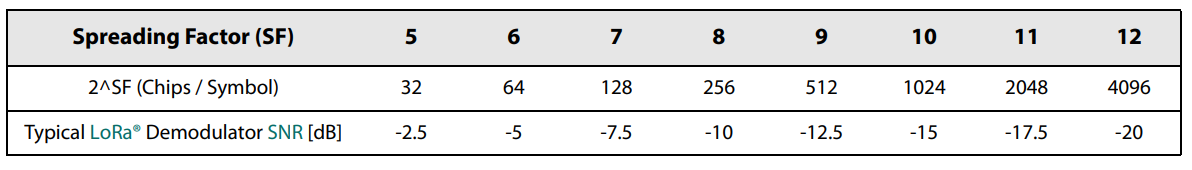
\includegraphics[width=\textwidth]{fig/semtech-sf-table.png}
    \caption{\label{table:semtech-sf}Range of Spreading Factors (SF).}
\end{figure}

Bandwidth variation exhibits similar traits, but to stay within the legal limits of the EU868 band, it is necessary to stay within $125\text{--}500~\mathrm{kHz}$ \cite{etsi_short_2018, thethingsnetwork_eu863-870_nodate}. This is the reason for selecting SF as the variable, while keeping the Bandwidth and the coding rate (CR) constant. CR also has a very predictable effect on the connection quality.

\subsection{Hypothesis}
It is expected the proximity to the ground will have high impact on the usable range of the sensor, meaning Nodes mounted with their antenna closer to the ground should perform worse. Higher SF should yield longer range. We are not expecting to surpass distance of $1~\mathrm{km}$.

\subsection{\label{section:range-prerequisite}Prerequisite}
The maximum achievable SF needed to be determined. This was done experimentally, starting with SF5 and incrementing util it was no longer possible to transfer data. This test was conducted using Nucleo acting as the initiator of connection with the LoRa module. Devices were situated on a desk about 1.5 meters apart with their antennae positioned orthogonally in respect to each other to avoid overwhelming the receiver. All other parameters are identical to those used in the latter experiment.

The connection was stable at SF11, but at SF12 the LoRa module stopped responding, thus the experiment was done at SF5 and SF11, which corresponds to a theoretical delta of $15~\mathrm{dB}$ \cite{semtech_corporation_sx12612_2024}.

\subsection{Methodology}
All LoRa modulation and packet parameters were set in firmware (commit \link{https://github.com/manakjiri/lora-module-fw/tree/76acdcd7b31f259c88f1808ed79886dc26295b4e}{76acdcd}) identically for all devices used, a summary is provided in Table \ref{table:range-test-parameters}. 

\begin{table}[H]
\begin{center}
\caption{\label{table:range-test-parameters}LoRa parameters for range testing.}
    \begin{tabular}{|l|l|} \hline
    Frequency             & $869.525~\mathrm{MHz}$\\ \hline
    RF power output       & $15~\mathrm{dBm}$\\ \hline
    Bandwidth             & $250~\mathrm{kHz}$\\ \hline
    Coding rate           & $4:8$ (2x overhead) \\ \hline
    Bandwidth             & $250~\mathrm{kHz}$\\ \hline
    Preamble length       & $32~\mathrm{b}$\\ \hline
    Implicit header       & No\\ \hline
    LoRa CRC              & No\\ \hline
    Inverted IQ           & No\\ \hline
    Transmit boost        & No\\ \hline
    Receive boost         & No\\ \hline
    \end{tabular}
\end{center}
\end{table}

LoRa modules used the MOLEX 105262--0003 antenna and Nucleo boards used their stock antenna, all were close to vertical orientation. A pole with two LoRa modules and one Nucleo (see Figure \ref{fig:range-nodes}) was constructed to act as the stationary set of Nodes to test against. Another Nucleo board was attached to a car (see Figure \ref{fig:range-gateway}) to act as the Gateway, see Table \ref{table:range-test-devices} for more details.

\begin{figure}[p]
    \centering
    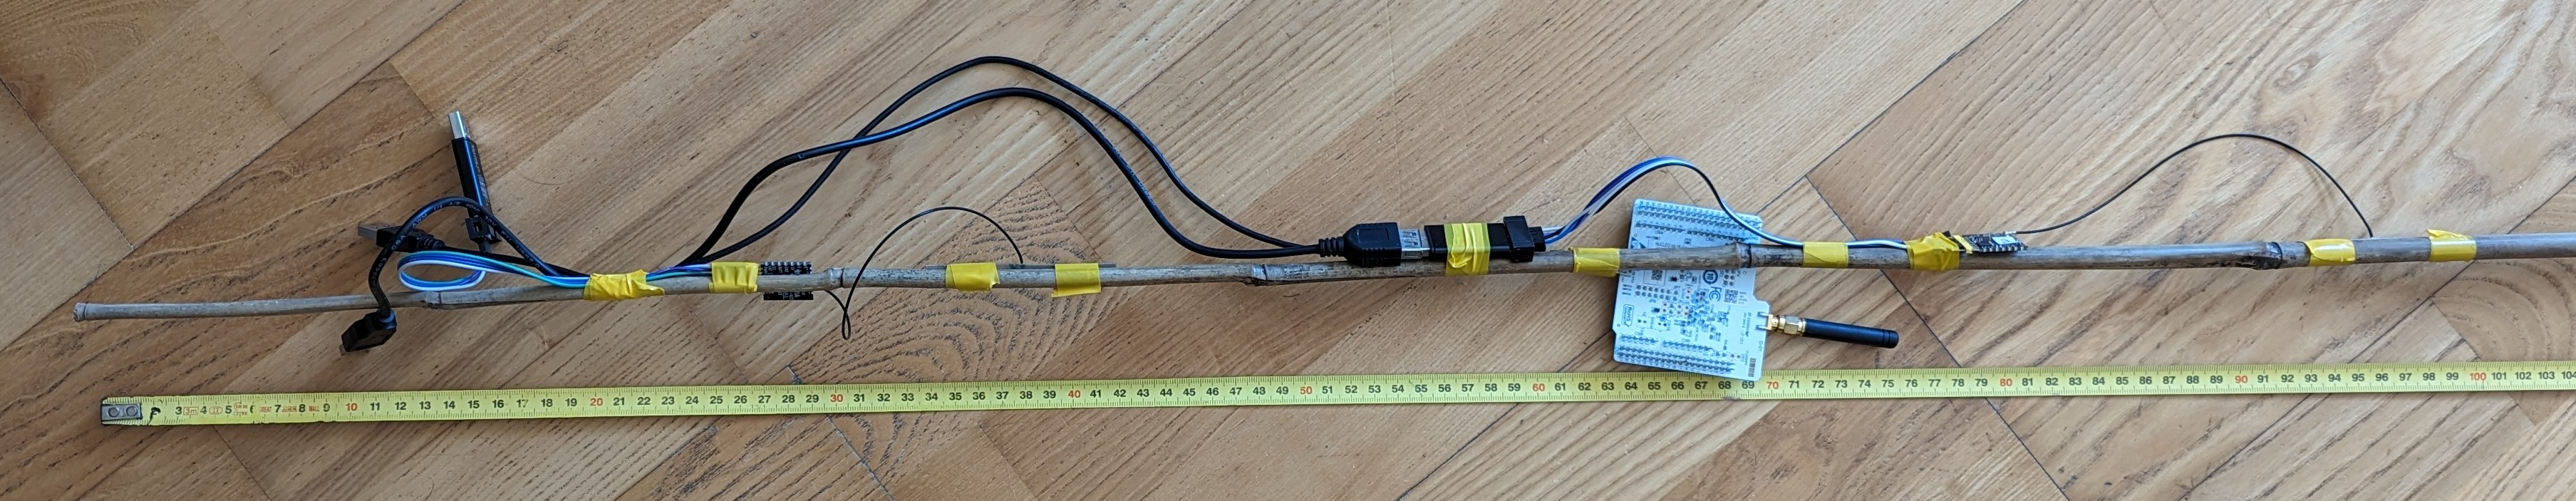
\includegraphics[width=.9\textwidth]{img/lora-pole.jpg}\vspace{1em}
    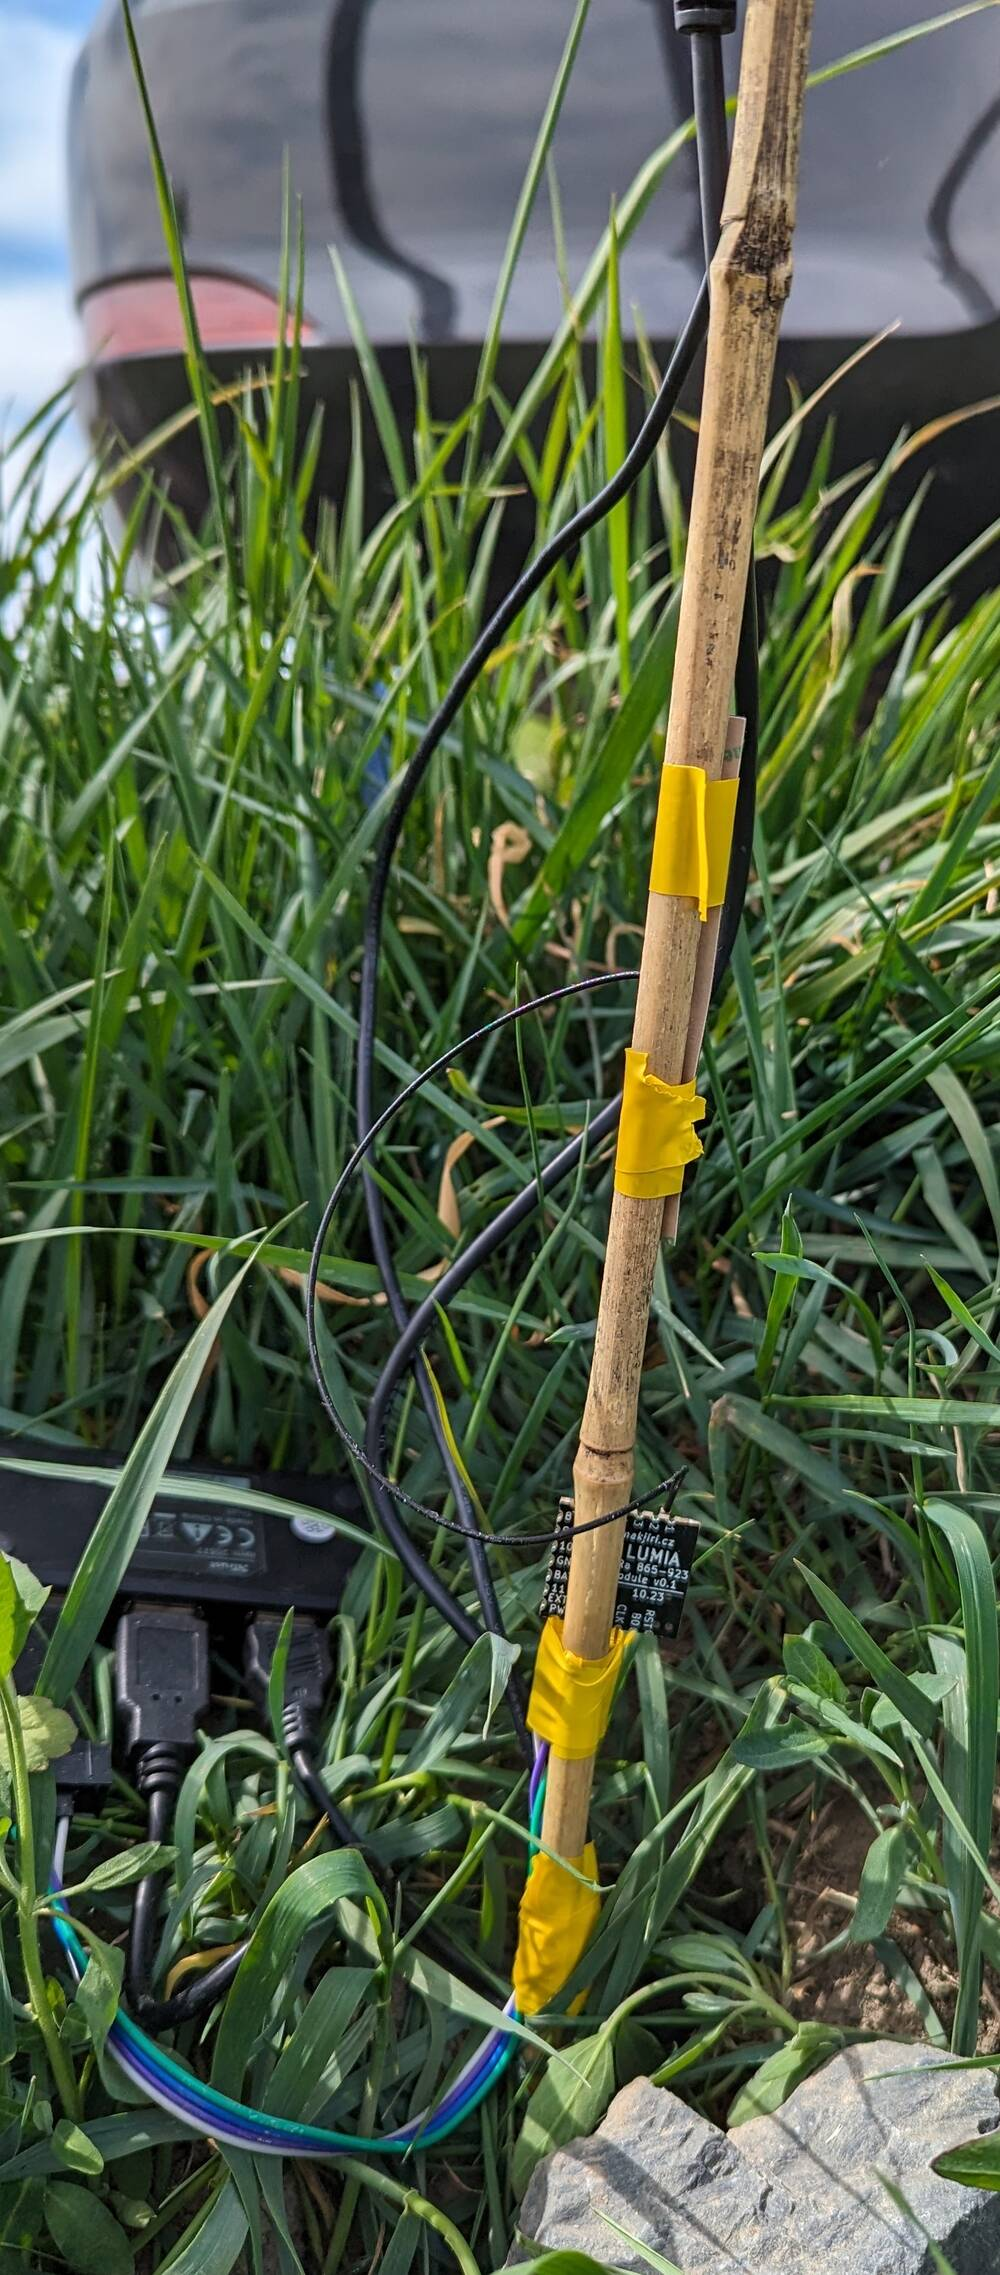
\includegraphics[width=.25\textwidth]{img/range-pole-base.jpg}\hfil
    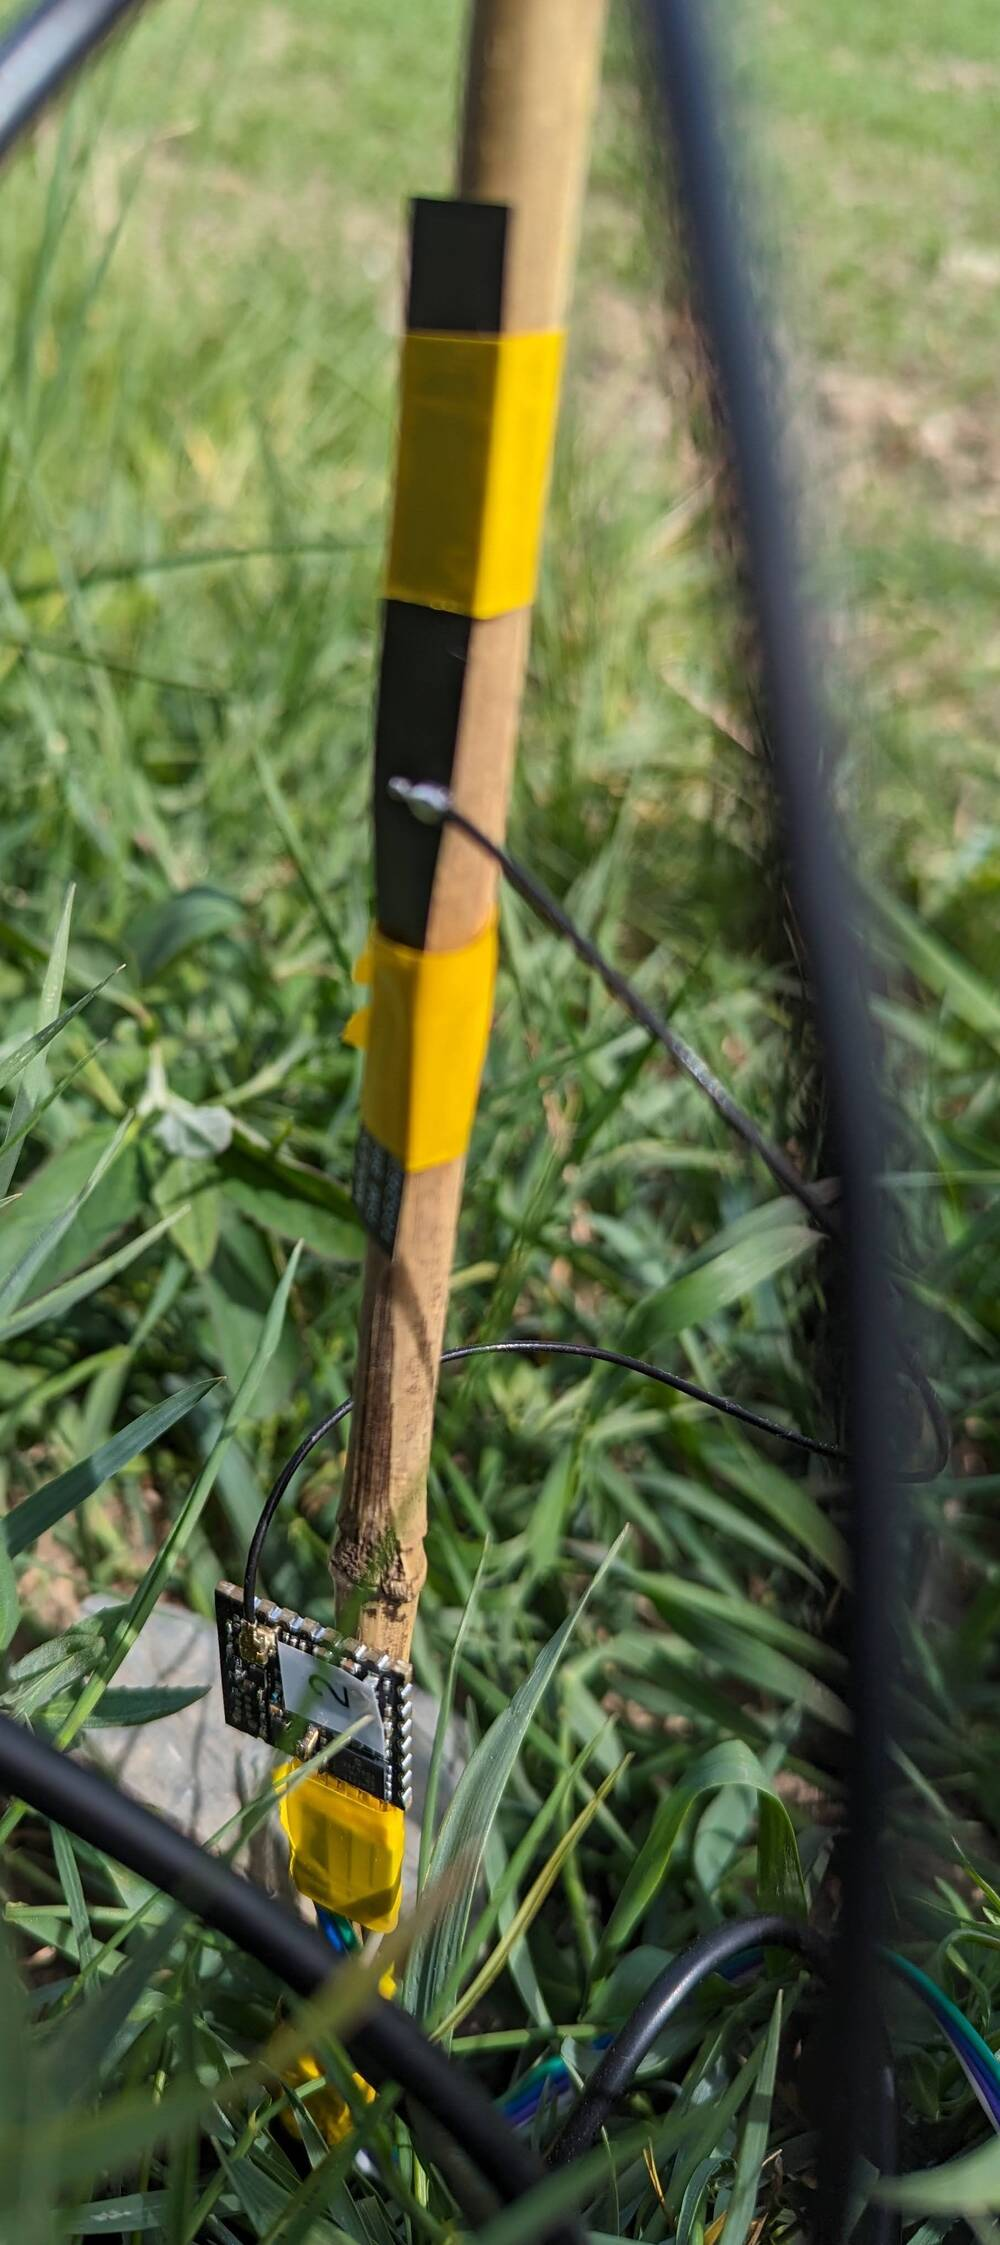
\includegraphics[width=.25\textwidth]{img/range-pole-bottom.jpg}\hfil
    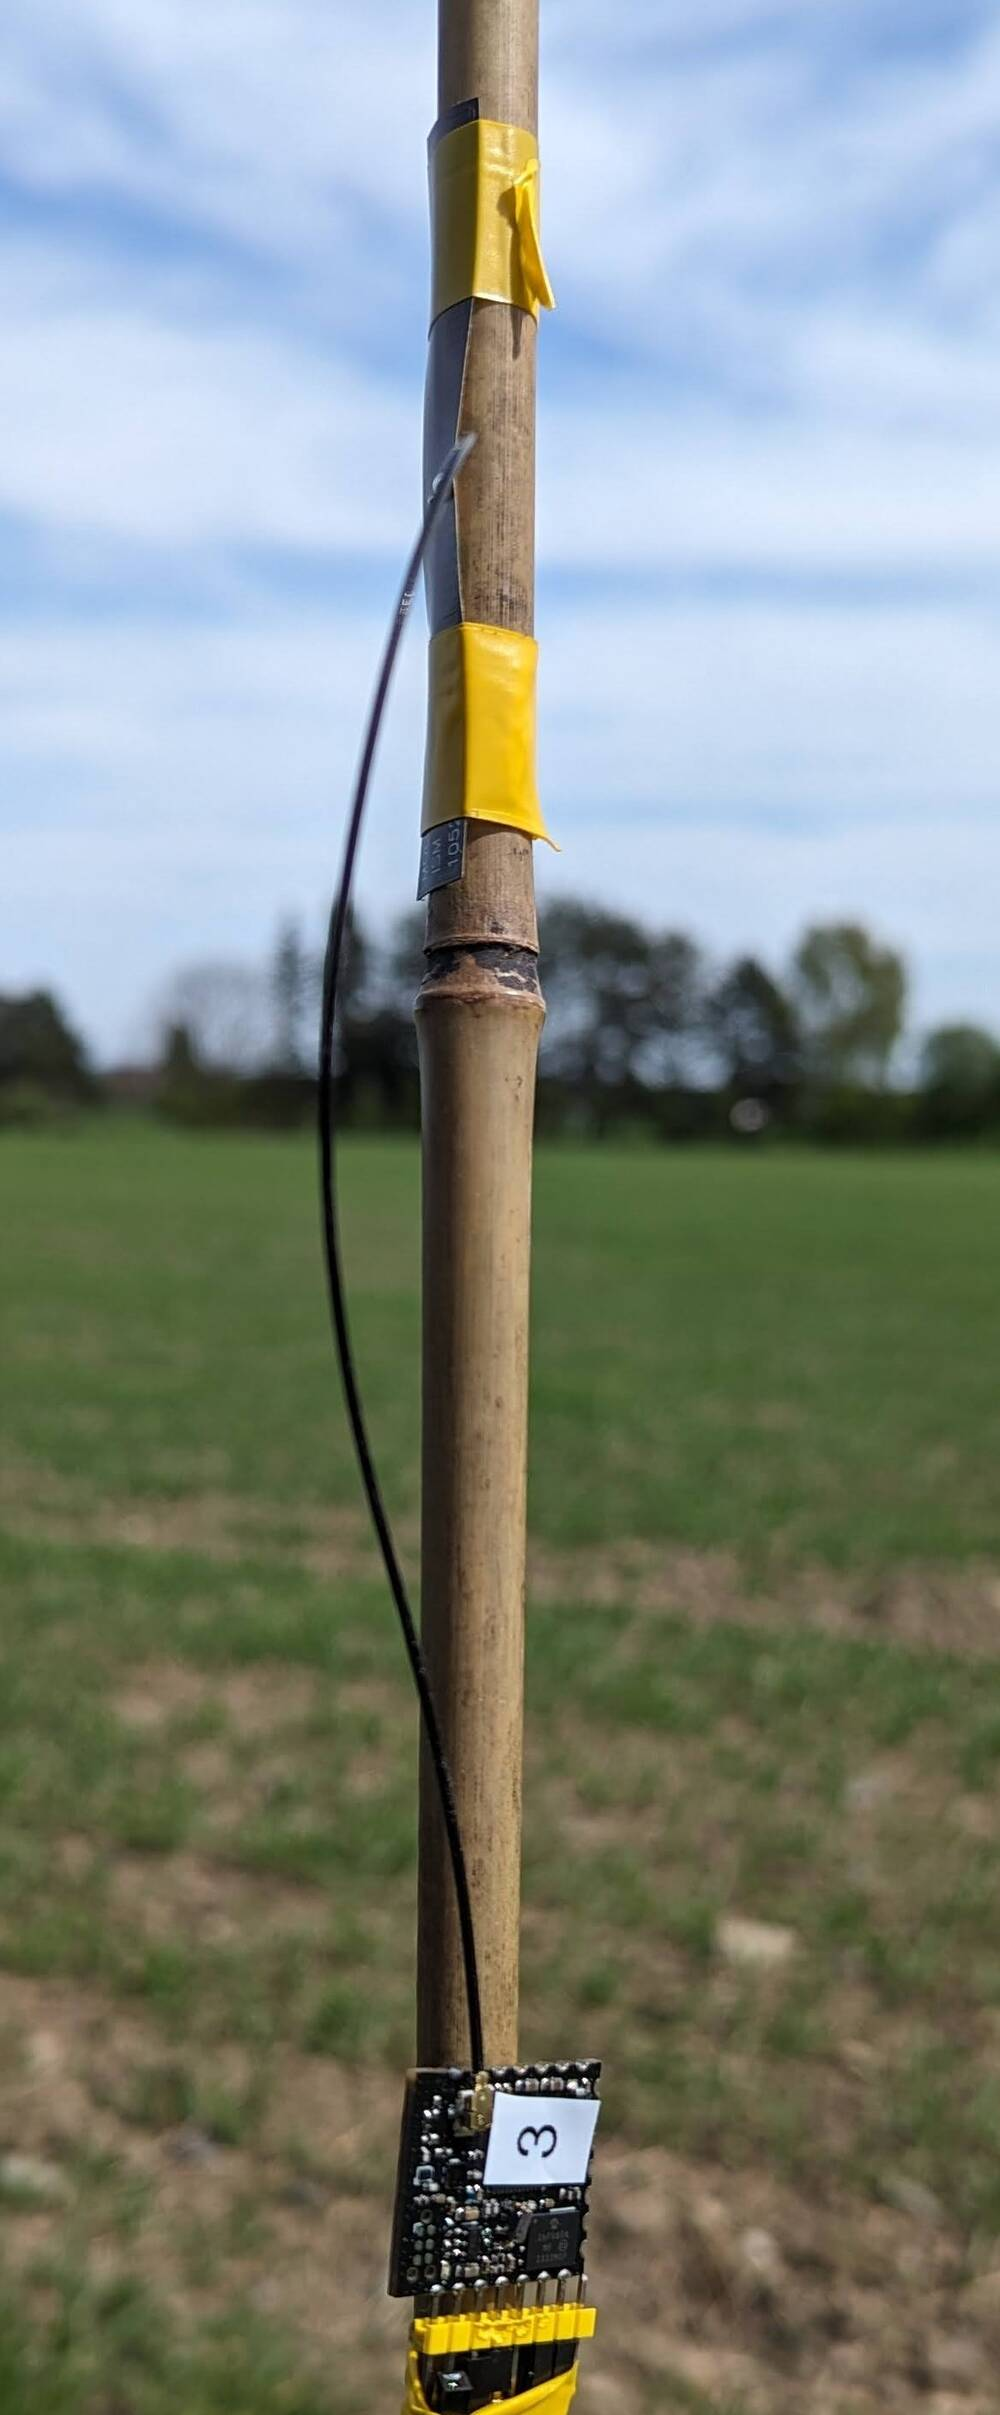
\includegraphics[width=.24\textwidth]{img/range-pole-top.jpg}
    \caption{\label{fig:range-nodes}Close-up of the pole with Nodes attached for range testing.}
\end{figure}

\begin{figure}[p]
    \centering
    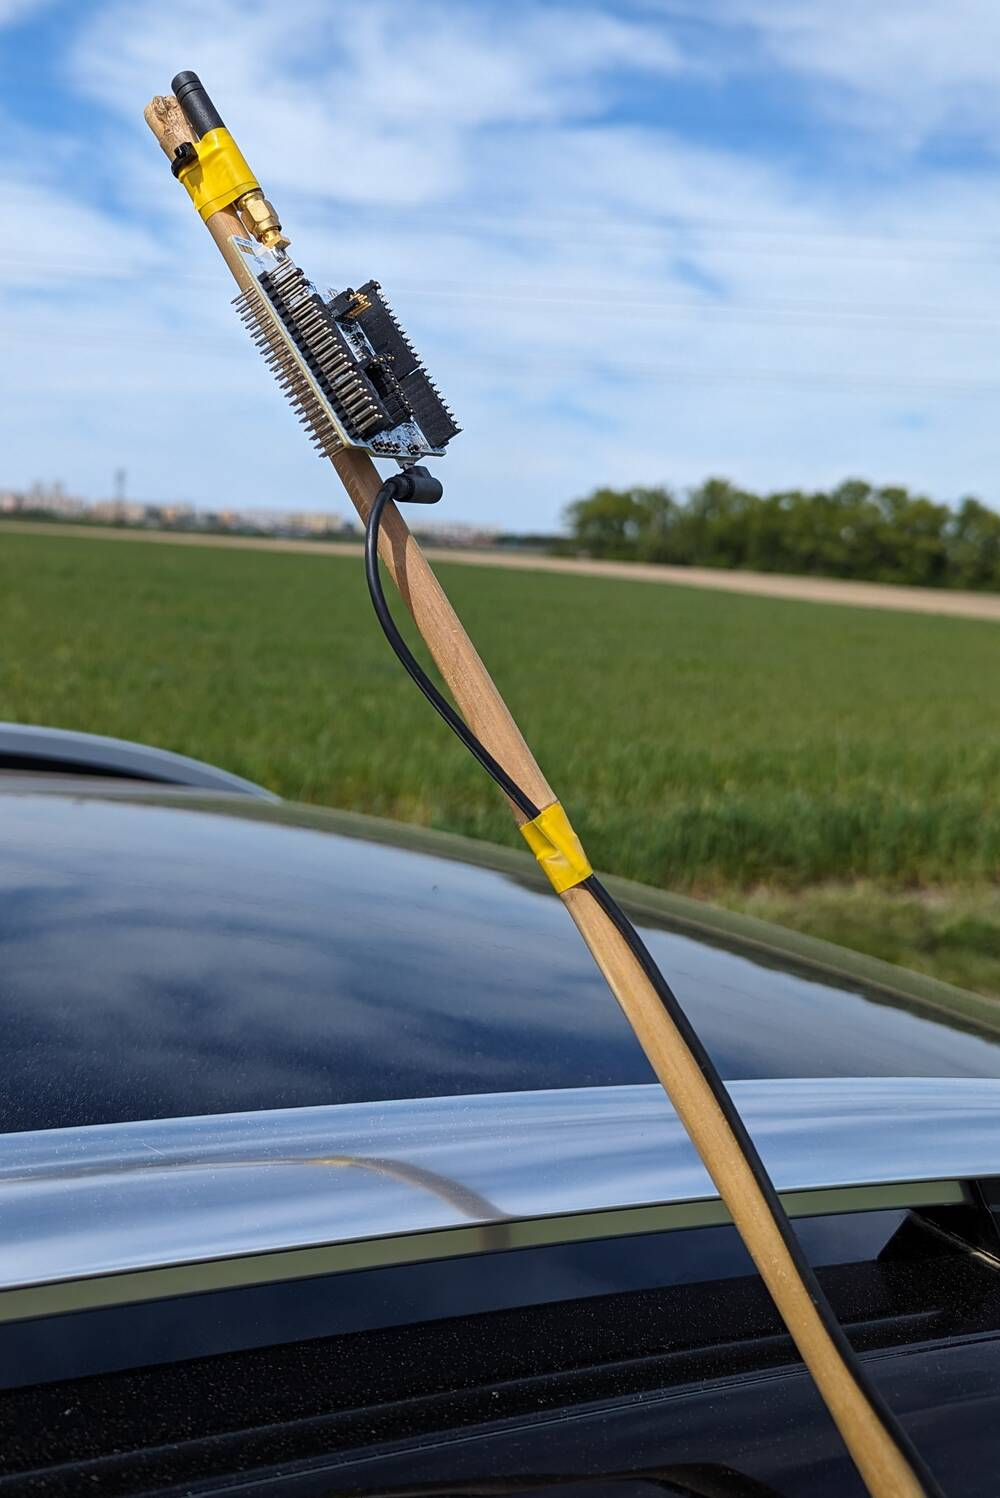
\includegraphics[width=.35\textwidth]{img/range-gateway1.jpg}\hfil
    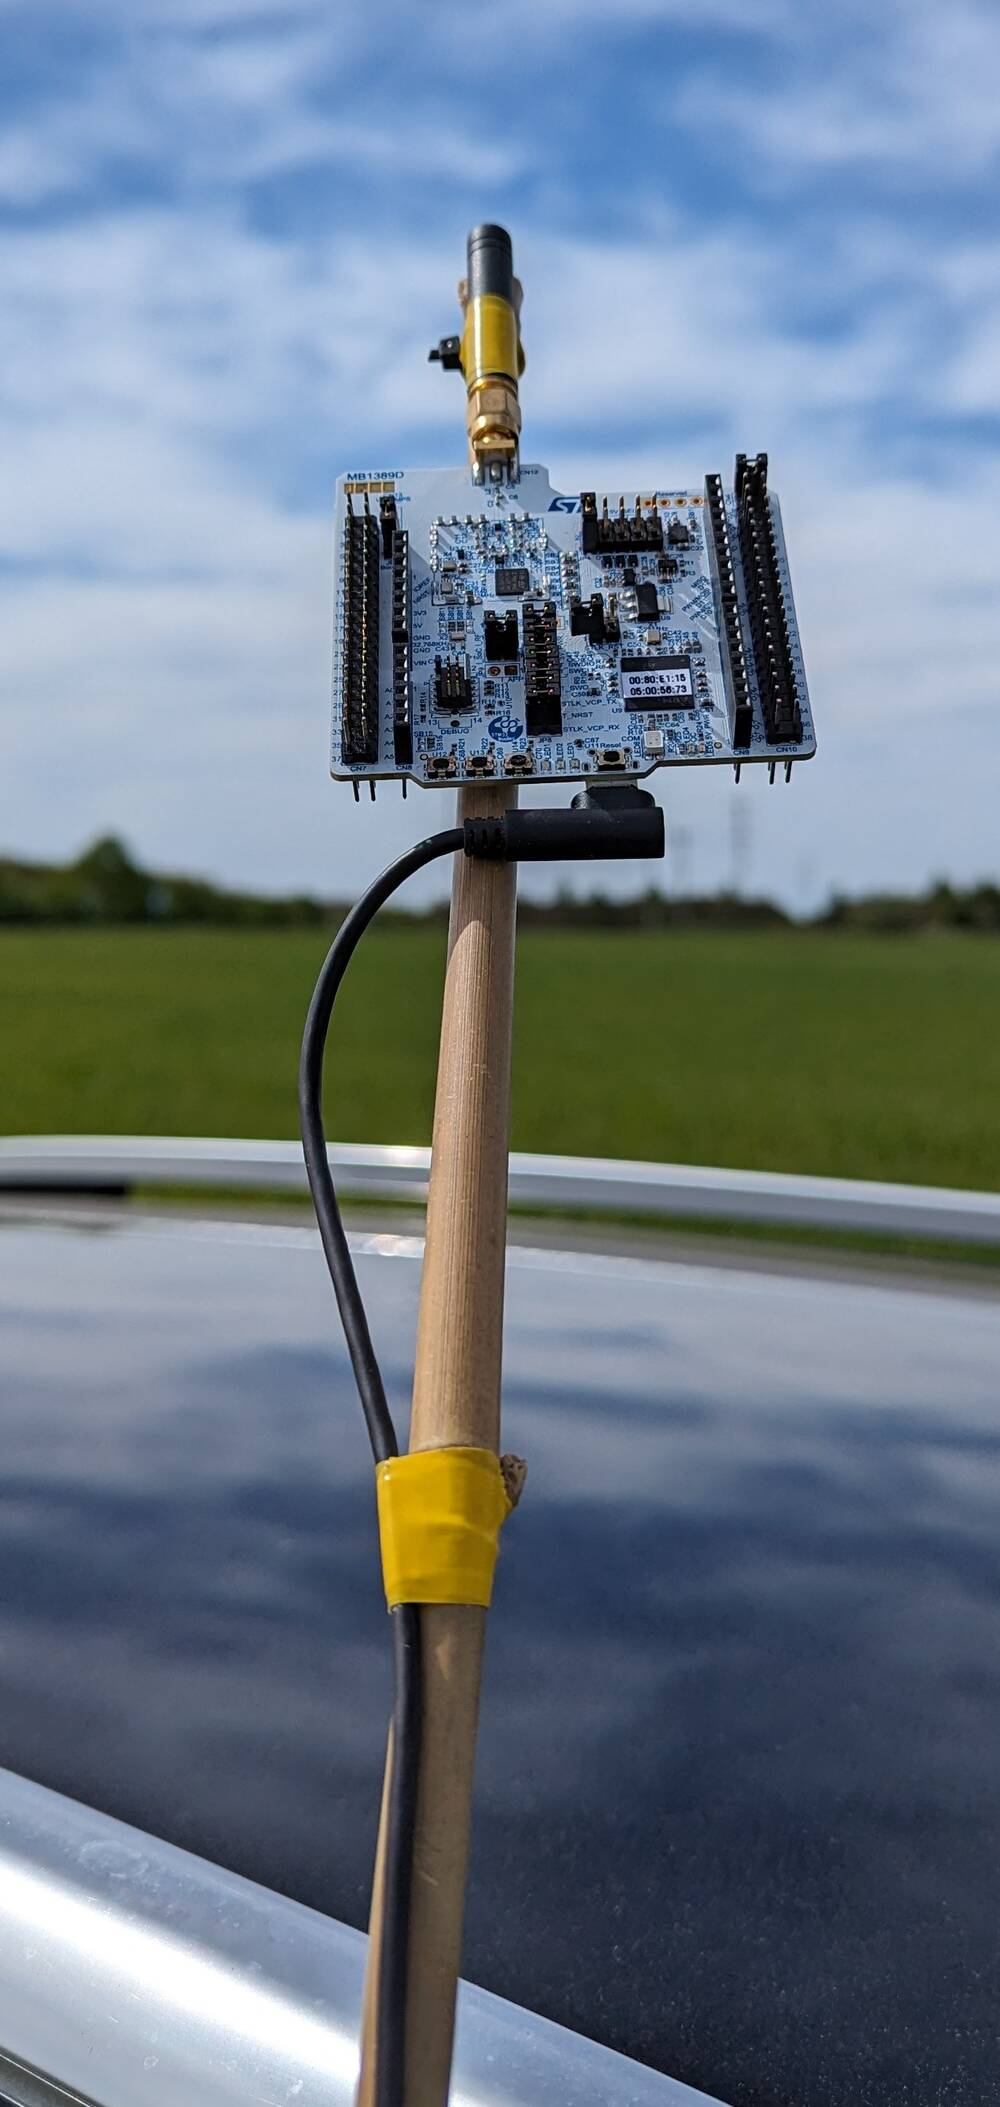
\includegraphics[width=.25\textwidth]{img/range-gateway2.jpg}
    \caption{\label{fig:range-gateway}Close-up of Nucleo attached to the car acting as the Gateway for range testing.}
\end{figure}

\begin{table}[H]
\begin{center}
\caption{\label{table:range-test-devices}Devices used for range testing.}
    \begin{tabular}{|l|l|l|} \hline
    \textbf{Device} & \textbf{Height\footnote{Measured distance from the root of the antenna to ground level} [m]} & \textbf{Address}\footnote{Data presented will use these addresses to distinguish between the different Nodes used in the experiment} \\ \hline
    Nucleo (Gateway) & 1.65 & 1 \\ \hline
    LoRa module (Node) & 0.19 & 2 \\ \hline
    Nucleo (Node) & 0.55 & 4 \\ \hline
    LoRa module (Node) & 0.82 & 3 \\ \hline
    \end{tabular}
\end{center}
\end{table}

A location was picked to represent the final use--case, a field with sections of direct line--of--sight (LOS) and sections obstructed by hills. This place is situated near Průhonice municipality in the Czech Republic. The pole with Nodes attached was installed at \href{https://en.mapy.cz/letecka?q=50.0012006N%2C%2014.5308962E&x=14.5381677&y=50.0011824&z=16}{50.0012006N, 14.5308961E}\footnote{https://en.mapy.cz/letecka?q=50.0012006N\%2C\%2014.5308962E\&x=14.5381677\&y=50.0011824\&z=16} (WGS84).

A set of measurements was taken through the Gateway at different locations progressing further from the stationary pole with the Nodes attached. These measurements consisted of downloading a random binary 1 KB file to each of the Nodes consecutively. This file was fragmented on the fly by the OTA update protocol to 16 blocks of 64 bytes each.

This means that effectively 16 different measurements of the signal quality were taken at each location for each of the three Nodes. Measurements were recorded by the system in a CSV file containing the time since download started, the amount of packets sent and the last block that was acknowledged - thus a success rate can be calculated. In case the download failed to initiate, nothing gets recorded and that is interpreted as 0\% success rate.

\subsection{Results}
As this is an experiment, where direct line--of--sight cannot be relied upon to interpret the results, it was deemed necessary to somehow capture the environment, the terrain, and present it along with the obtained data.

Altitude data was obtained from the \link{https://api.mapy.cz/v1/elevation}{Seznam.cz elevation API} in 5 m resolution of interpolated coordinates of lines connecting the Nodes and Gateway locations. This location data is also available in raw form as part of the Appendix \ref{chapter:more-range-test}.

\subsubsection{\label{section:edsl-definition}Elevation Deviation from the Straight Line}
Following graphs describe the terrain in terms of Elevation Deviation from the Straight Line (EDSL) connecting the Nodes location (spot 0) with the furthest point at which the last measurement was taken. Units of EDSL proportionally translate to meters, since the effect is similar to subtracting the offset signal in data.

The same data without the EDSL interpretation is included as Appendix \ref{chapter:more-range-test} for completeness. It also demonstrates the need for such data manipulation, because the features of the terrain are a lot less apparent in the original data.

\begin{figure}[p]
    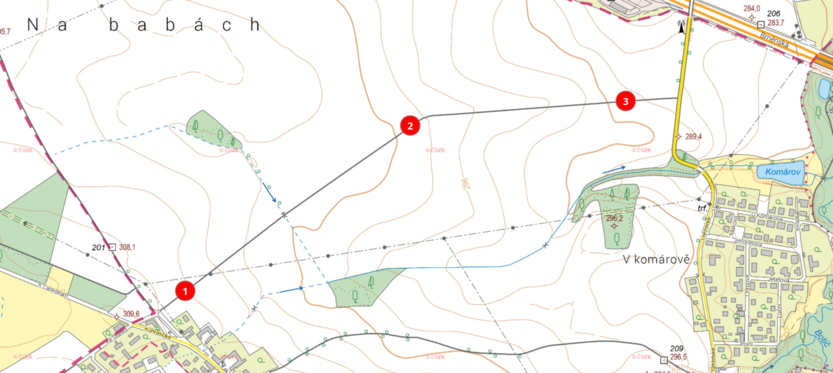
\includegraphics[width=.9\textwidth]{img/range-test-map.png}
    \caption{\label{fig:range-test-map}Map of the range test site. Correlation with Figures \ref{fig:range-relief} and Table \ref{table:range-results} follows: point 1 corresponds to the Nodes location (spot 0), point 2 is the spot 5 in both SF5 and SF11 measurements, point 3 is the spot 9 and spot 11 for SF11 and SF5 respectively. Source: \href{https://ags.cuzk.cz/geoprohlizec}{Geoprohlížeč ČÚZK}.}
\end{figure}

\subsubsection{Effect of the Spreading Factor}
Lower SF decreases the packet air time at the expanse of lower range reached. SF5 averaged $0.125~\mathrm{s}$, while SF11 averaged $1.125~\mathrm{s}$ round-trip time (excluding packet-loss) with these payloads.

Using SF5, it was possible to maintain stable connection with Nodes (3 and 4) positioned higher above the ground level even when occluded by the terrain. Connection with Node 2 was lost as soon as any occlusion was introduced. It can be expected that this setup would be feasible in very flat environments, but could be susceptible to dropouts with slight changes, such as growing crops.

The SF11 configuration exceeded expectations in terms of distance reached, a stable connection was maintained with all Nodes without difference in packet loss, which is perhaps most surprising, since some degradation was expected at least for the Node 2 position closest to the ground level. 

While the range was higher than with SF5, the connection quality is somewhat worse in the stable regions (less than 500 m distance, direct line-of-sight) for SF11. This suggests that a stability limit was indeed reached, as alloted to in the Prerequisite Section \ref{section:range-prerequisite}.

\begin{figure}[p]
    \centering
    \subfloat[SF11]{\includesvg[width=0.95\textwidth]{data/range/out/relief-sf11.svg}} \hfil
    \subfloat[SF5]{\includesvg[width=0.95\textwidth]{data/range/out/relief-sf5.svg}}
    \caption{\label{fig:range-relief}Graph of the range test locations, their distance from the pole with Nodes, and the relief in the path of the signal described as Elevation Deviation from the Straight Line \ref{section:edsl-definition}, which compensates the downward slope of the terrain and brings attention to the features of the terrain. Black crosses signify the position of the antennae of each device for each spot number.}
\end{figure}

\begin{figure}[p]
    \centering
    \subfloat[SF11]{\includesvg[width=\textwidth]{data/range/out/success-sf11.svg}} \hfil
    \subfloat[SF5]{\includesvg[width=\textwidth]{data/range/out/success-sf5.svg}}
    \caption{\label{fig:range-results}Graph of the packet transfer success rate for each Node with respect to the transmission distance.}
\end{figure}

\begin{figure}[p]
\begin{minipage}[t]{.45\textwidth}
    \vspace{0pt}
    \begin{tabular}{|l|l|l|l|}
\multicolumn{4}{c}{\textbf{SF11}} \\ \hline 
\textbf{Spot} & \textbf{Node 4} & \textbf{Node 3} & \textbf{Node 2} \\ \hline
0 & 100\% & 100\% & 100\% \\ \hline
1 & 100\% & 100\% & 100\% \\ \hline
2 & 100\% & 94\% & 100\% \\ \hline
3 & 100\% & 100\% & 100\% \\ \hline
4 & 100\% & 100\% & 100\% \\ \hline
5 & 100\% & 94\% & 100\% \\ \hline
6 & 100\% & 100\% & 94\% \\ \hline
7 & 100\% & 100\% & 100\% \\ \hline
8 & 94\% & 100\% & 100\% \\ \hline
9 & 100\% & 94\% & 100\% \\ \hline
\end{tabular}

\end{minipage}
\begin{minipage}[t]{.45\textwidth}
    \vspace{0pt}
    %\begin{table}
        \begin{tabular}{|l|l|l|l|}
\multicolumn{4}{c}{\textbf{SF5}} \\ \hline 
\textbf{Spot} & \textbf{Node 4} & \textbf{Node 3} & \textbf{Node 2} \\ \hline
0 & 100\% & 100\% & 100\% \\ \hline
1 & 100\% & 100\% & 100\% \\ \hline
2 & 100\% & 100\% & 100\% \\ \hline
3 & 100\% & 100\% & 100\% \\ \hline
4 & 100\% & 100\% & 100\% \\ \hline
5 & 100\% & 100\% & 100\% \\ \hline
6 & 100\% & 100\% & 100\% \\ \hline
7 & 100\% & 100\% & 0\% \\ \hline
8 & 100\% & 100\% & 0\% \\ \hline
9 & 100\% & 100\% & 0\% \\ \hline
10 & 89\% & 0\% & 0\% \\ \hline
11 & 89\% & 100\% & 0\% \\ \hline
\end{tabular}
    
    %\end{table}
\end{minipage}
\caption{\label{table:range-results}Success rates for each node and location at spreading factors 5 and 11.}
\end{figure}

\begin{figure}[p]
    \centering
    \begin{minipage}[t]{\textwidth}
        \centering
        \begin{tabular}{|l|l|l|l|}
\multicolumn{4}{c}{\textbf{SF11-FAR1}} \\ \hline 
\textbf{Spot} & \textbf{Node 4} & \textbf{Node 3} & \textbf{Node 2} \\ \hline
0 & 100\% & 100\% & 100\% \\ \hline
10 & 100\% & 6\% & 0\% \\ \hline
\end{tabular}

        \vspace{1em}
    \end{minipage}
    \includesvg[width=\textwidth]{data/range/out/relief-sf11-far1-lines.svg}
    \caption{\label{fig:range-relief-far1}Table of the success rates and graph of the first long range test location, distance from the pole with Nodes, and the relief in the path of the signal described as Elevation Deviation from the Straight Line \ref{section:edsl-definition}, which compensates the downward slope of the terrain and brings attention to the features of the terrain. Black crosses signify the position of the antennae of each device for each spot number. Dashed lines highlight the direct line-of-sight for the antennae.}
\end{figure}

\begin{figure}[p]
    \centering
    \begin{minipage}[t]{\textwidth}
        \centering
        \begin{tabular}{|l|l|l|l|}
\multicolumn{4}{c}{\textbf{SF11-FAR2}} \\ \hline 
\textbf{Spot} & \textbf{Node 4} & \textbf{Node 3} & \textbf{Node 2} \\ \hline
0 & 100\% & 100\% & 100\% \\ \hline
11 & 100\% & 100\% & 100\% \\ \hline
\end{tabular}

        \vspace{1em}
    \end{minipage}
    \includesvg[width=\textwidth]{data/range/out/relief-sf11-far2-lines.svg}
    \caption{\label{fig:range-relief-far2}Table of the success rates and graph of the second long range test location, distance from the pole with Nodes, and the relief in the path of the signal described as Elevation Deviation from the Straight Line \ref{section:edsl-definition}, which compensates the downward slope of the terrain and brings attention to the features of the terrain. Black crosses signify the position of the antennae of each device for each spot number. Dashed lines highlight the direct line-of-sight for the antennae.}
\end{figure}

\subsubsection{Maximum Distance}
Finding the limit at FS11 proved to be more difficult than anticipated. The surrounding environment either contained too favorable, or absolutely unfavorable conditions at further distances. Two additional data points displayed in Figures \ref{fig:range-relief-far1} and \ref{fig:range-relief-far2} were gathered at locations outside of the planed path.

The first Figure \ref{fig:range-relief-far1} shows the only flawless connection with the Nucleo Node 4, which must have been facilitated thanks to a signal reflection from some other feature in the environment. While the connection with Node 3 was initiated and it acknowledged 2 packets, the connection later timed out after the Node failed to respond in 30 more attempts.

The second location, captured by Figure \ref{fig:range-relief-far2}, exhibited flawless transmission of the payload for all 3 Nodes at a distance of 1.2 km with occlusion.

The nature of LoRa is that it performs well within its large link budget, but once that is exhausted, the performance drops off rapidly. The attenuation of the medium through which the electromagnetic wave travels changes with temperature and saturation with humidity and particulate, the position of the antennae may change slightly due to wind and the onboard oscillators can drift with temperature and power supply.

Most of these factors remained constant throughout this experiment, since it was done within a 1.5 hour window, but must be considered for long-term deployments.

\section{\label{section:sensor-validation}Soil Moisture Sensor Validation}
A practical experiment was conducted to validate the functioning of the soil moisture sensor itself.

\begin{figure}
    \centering
    \subfloat[\label{fig:case}CAD design render of the soil moisture sensor case (bottom left) including the hinge providing the sviwel adjustment of the panel (center) and the panel plate part.]{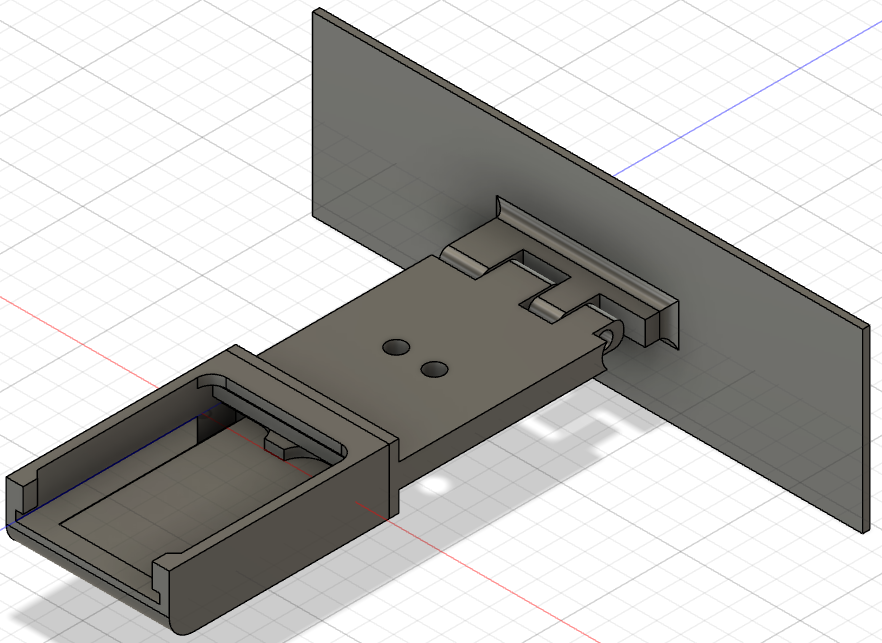
\includegraphics[width=.44\textwidth]{img/sensor-case.png}} \hfill
    %\subfloat[Illustrative picture]{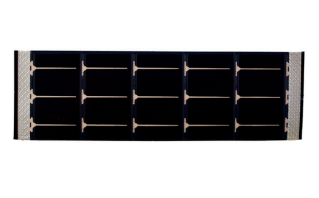
\includegraphics[width=.39\textwidth,angle=90]{img/panel.png}} \hfill
    \subfloat[\label{fig:panel}IV Curve of the MP3-37 solar panel manufactured by PowerFilm, which was used for the soil moisture sensor validation.]{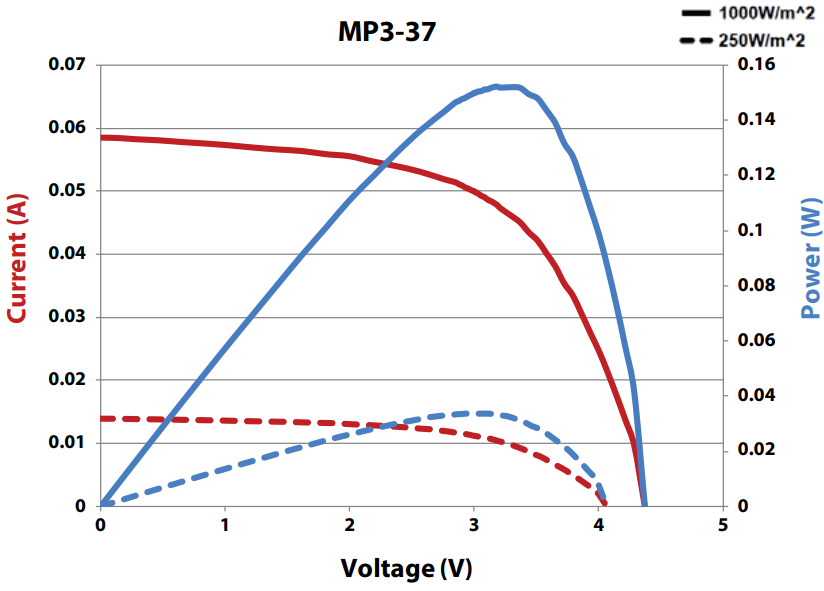
\includegraphics[width=.54\textwidth]{fig/panel-iv.png}}
    \caption{Soil moisture sensor case (left) and the IV curve of the solar panel (right). Both parts were used during the soil moisture sensor validation.}
\end{figure}

\begin{figure}
    \centering
    \subfloat[Soil moisture sensor stuck in the pot (center) on a window sill facing south. The lithium battery is connected externally through the RaspberryPi Pico development board (bottom), acting as a data logger of the voltage and current.]{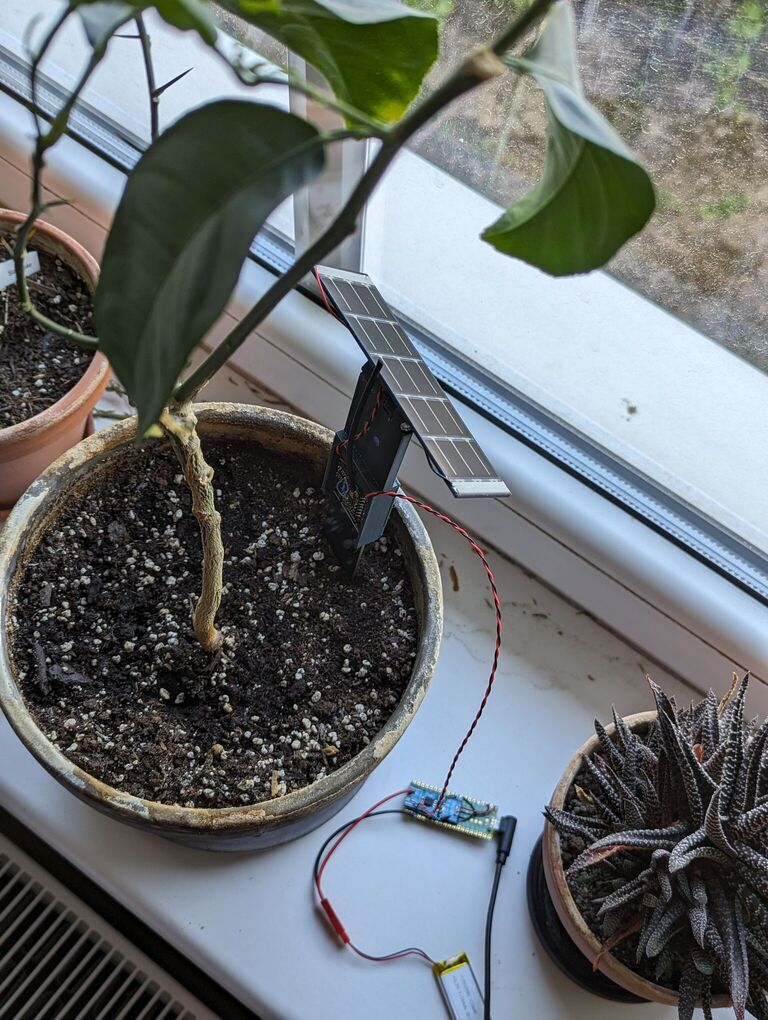
\includegraphics[width=.45\textwidth]{img/sensor-deploy-up.jpg}} \hfil
    \subfloat[Close--up picture of the sensor and its housing. The LoRa module is clearly visible, along with the conncetions to the solar panel, the battery and the antenna.]{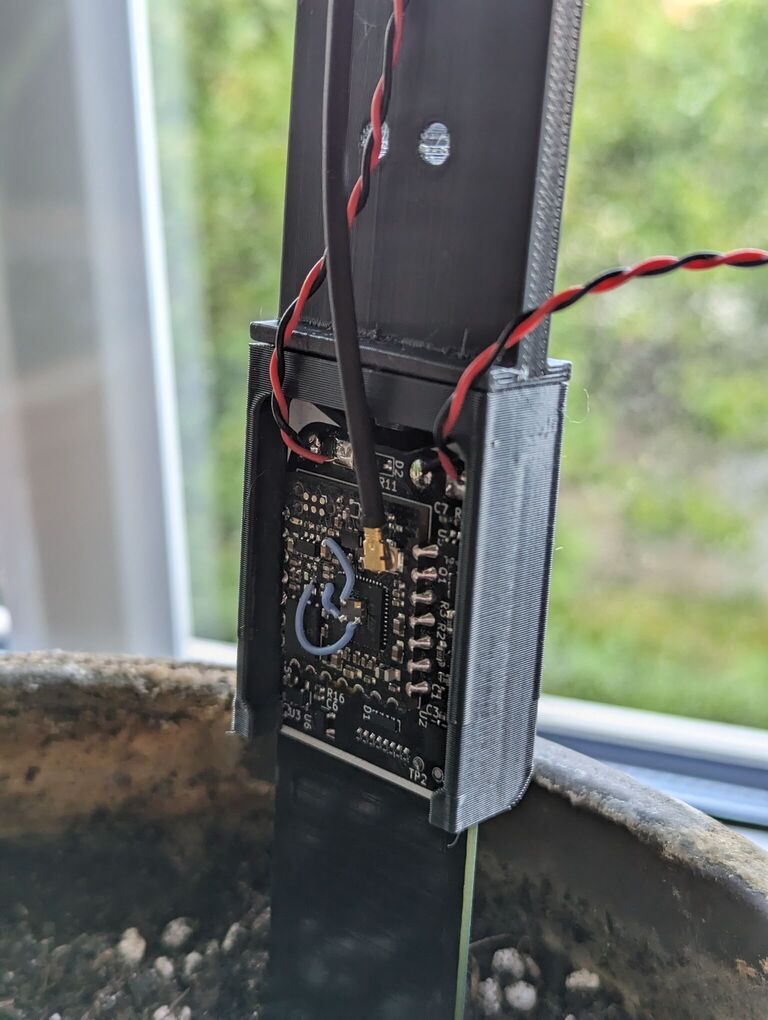
\includegraphics[width=.45\textwidth]{img/sensor-deploy-close.jpg}}
    \caption{\label{fig:sensor-deploy}Soil moisture sensor proof--of--concept deployment scenario used for validating the solar panel performance and the sensor's measuring capabilities.}
\end{figure}

\subsection{Hypothesis}
The sensor should detect soil moisture based on the experiments done during sensor validation. It is also expected that the sensor will be able to charge its battery when enough sunlight is available.

\subsection{Prerequisite}
The sensor is meant to be made self--sufficient thanks to a solar panel. The main constraint is the power generated and the panel's dimensions. Since the solar panel is charging the battery directly, it needs to generate sufficiently high voltage to do so. The MP3--37 from PowerFilm was picked, because its open circuit voltage is 4.6 V, and according to \ref{fig:panel}, it should produce 50 mA at 4.1 V, which is ideal for this application.

%https://cz.mouser.com/datasheet/2/1009/Electronic_Component_Spec_Sheet_Cla_77DEA84523C82-1658524.pdf

A sensor housing needed to be constructed to support the solar panel in the correct orientation. The housing was designed in Fusion 360 CAD software and 3D printed, as visible in Figure \ref{fig:sensor-deploy}. The housing has a support arm for the solar panel, which allows it to swivel, which is better viewed in Figure \ref{fig:case}.

Lastly, the sensor's scale needed to be calibrated. This was done by taking 10 measurements in free air (Dry) and fully submerged in water (Wet). The resulting coefficients are included in Table \ref{table:sensor-calibration}. These coefficients are used for calculating the soil moisture saturation using the following equation
\begin{equation}
    \theta' = \dfrac{T - T_{Dry}}{T_{Wet} - T_{Dry}}
\end{equation}

\begin{table}
\begin{center}
\caption{\label{table:sensor-calibration}Soil moisture sensor zone calibration coefficients.}
    \begin{tabular}{|l|l|l|l|} \hline
    \textbf{Zone} & \textbf{Depth [mm]} & \textbf{Dry value [$\mu$s]} & \textbf{Wet value [$\mu$s]} \\ \hline
    1 & 20 & 276 & 728 \\ \hline
    2 & 50 & 277 & 728 \\ \hline
    3 & 90 & 277 & 581 \\ \hline
    4 & 120 & 277 & 498 \\ \hline
    \end{tabular}
\end{center}
\end{table}

\subsection{Methodology}
The sensor was stuck in the existing planter of a citrus tree plant. Sensor readings are gathered using the LoRa interface every 15 seconds. Power logger readings using Raspberry Pi Pico are also gathered every 15 seconds. 

The power logger is measuring the battery voltage and current. Thus any power consumed by the sensor itself during charging is not visible, but is assumed to be constant throughout the experiment, as the reading interval is fixed.

The planter with the sensor is placed behind a glass window facing south. The panel is inclined by the swivel mechanism at about 30 degrees.

\subsection{Results}
\begin{figure}[p]
    \includesvg[width=\textwidth]{data/deployment/out/moisture-cal.svg}
    \caption{\label{fig:sensor-log}Filtered readings from the individual sensor zones. Zone 1 (green) is in free air acting as control (as can be seen in Figure \ref{fig:sensor-deploy}), zones 2 and 3 below it (brown and purple) are completely submerged in the soil. Zone 4 (magenta) is in the boundary layer of soil and Ceramsite at the bottom of the pot. The sample was watered 7 days before the marked point of watering (sharp increase), after which a decline in the measured capacitance can be observed, corresponding to the sample drying out. The sensor run out of power during the night, these areas are highlighted in grey.}
\end{figure}
\begin{figure}[p]
    \includesvg[width=\textwidth]{data/deployment/out/power.svg}
    \caption{\label{fig:power-log}Battery voltage (black) and charging power (yellow), excluding the power consumed by the sensor and the module itself. The power is provided solely by the 150 mWp solar panel. The experiment was started with the battery completely empty. Voltages below 2.8 V are left out, the under--voltage protection of the sensor always triggered at 2.5 V}
\end{figure}

The sensor was started on external power supply the day prior to the test to gather the initial measurements visible in the Figure \ref{fig:sensor-log} up to 12.5 00:00. After enough readings were gathered, the sensor was connected to its 330 mAh Lithium Polymer battery, which has been discharged completely prior to the experiment. The soil was mostly dry, as can be seen in the referenced Figure.

Watering occurred at 12.05 10:10, at which point the relative moisture saturation started raising into the 60--80 percent range in all but the control zone. The soil moisture was than gradually dropping throughout the following 7 days. Notably the surface zone (zone 2, brown in Figure \ref{fig:sensor-log}) returned to the level of soil moisture saturation before the watering, whereas the root--level zones were drying slower, signaling that there is still enough moisture.

Figure \ref{fig:power-log} starts at the moment of power--on of the sensor in the morning the following day. The power consumption of the sensor was too high and the charging efficiency too poor for the sensor to maintain stable operation, as it discharged after midnight the following day at 2.5 V, at which point the sensor's battery protection circuitry disconnected it. Same event repeated at the same voltage all following days and is thus left out. It was overcast with occasional full sun the day of 12$^{th}$ of May, following two days offered full sun throughout.

At this point a problem was noticed by observing the data, where it was apparent that the sensor stopped charging even though there was full, unobstructed sun hitting the solar panel. This was rectified in the morning the following day (14$^{th}$ of May) by bypassing the charging diode D2 (see Figure \ref{schematic:sensor-1}). This caused a temporary disruption in the logged results, which manifested by the peak visible at roughly noon that day.

After this modification, the battery managed to reach higher voltage and the sensor stayed working longer than any previous day. The rest of the data is cyclical in the same way, thus not shown. This poor battery performance is caused by a combination of many factors:
\begin{itemize}
    \item Due to the hardware design mistake involving the crystal oscillator on the LoRa module \ref{fig:tcxo-bodge}, the TCXO cannot be switched off, which causes a constant current draw of 2.5 mA. The MCU has a capability to start the oscillator only when needed, which is implemented in the following revision of the LoRa module.
    \item The measuring interval is rapid to bring more data into understanding the sensor performance, which is not necessary for final deployment, where a measuring interval of 10 minutes or longer would suffice.
    \item The MCU is not able to run at low enough clock speed because of limitations in the firmware
    \item The solar panel is behind a double-glazed window with low solar zenith angle (summer solstice), causing some energy loss in the glass. Because of this, the solar panel may not be receiving enough radiation to reach peak performance, which would be expected given the clear sky.
    \item The battery is directly charged by the solar panel without any energy harvesting optimizations, like Maximum Power Point Tracking implemented. However this was a conscious decision during the sensor design to make it simple, at the cost of some efficiency.
    \item Lastly, the solar panel is obstructed by building and window features, which limit the irradiation time.
\end{itemize}
